\section{Topic Tree}
\subsection{Overview}
Most learning management systems do not have a simple and easy method to import course material and resources from other courses. Some LMS platforms such as OpenLearning have no method of importing any data at all, and other platforms such as Canvas allows you to import crowd sourced material into your own course, however still does not allow you to import topics of resources. \\

This new LMS will have a new topic tree feature, which will allow teachers and academics to add course material under a specific topic instead.\\
Each topic will have prequisites of other topics, for example the topic Graphs will be a prequisite for the topic Depth first Search.\\

\textbf{Topics}
A topic is a collection of course material that is related to a particular subject. For example, in UNSW's Introduction to Programming course (COMP1511), one of the topics in the course is "Pointers", which contains all course material related to pointers. Instructors can choose what constitutes as a topic, but a topic in this case is part of the course material of an entire course - it does not constitute all the course material of a single course. For example, there is no topic called "Introduction to Programming" or "COMP1511" as that is virtually unusable as not all of this content would be imported into another course.


\begin{figure}[h!]
    \centering
    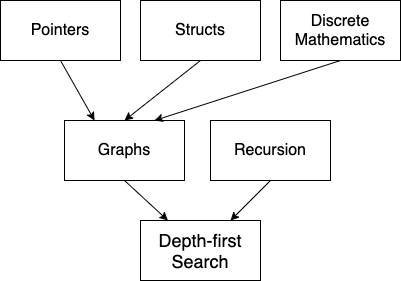
\includegraphics[scale=0.4]{topic-tree-example}
    \caption{Example of a topic tree with Depth first search}
\end{figure}

In the above example, pointers, structs and discrete mathematics must be learned in order to learn graphs. Likewise, graphs and recursion is required to learn depth first search.\\


Specific courses in this new LMS would be created by choosing the topics this new course has, and all course materials under each topic would be imported into the respective topic. This allows for faster creation of courses, and course materials can be reused more easily.\\

\subsection{UI/UX}
Instead of only a graph view, we opted for a more traditional UI for the topic tree as well. This is because a graph based UI may be unstable and difficult to use compared to a more traditional UI.\\

The following is a mockup of a possible UI, and will be changed in the future.\\
\begin{figure}[h!]
    \centering
    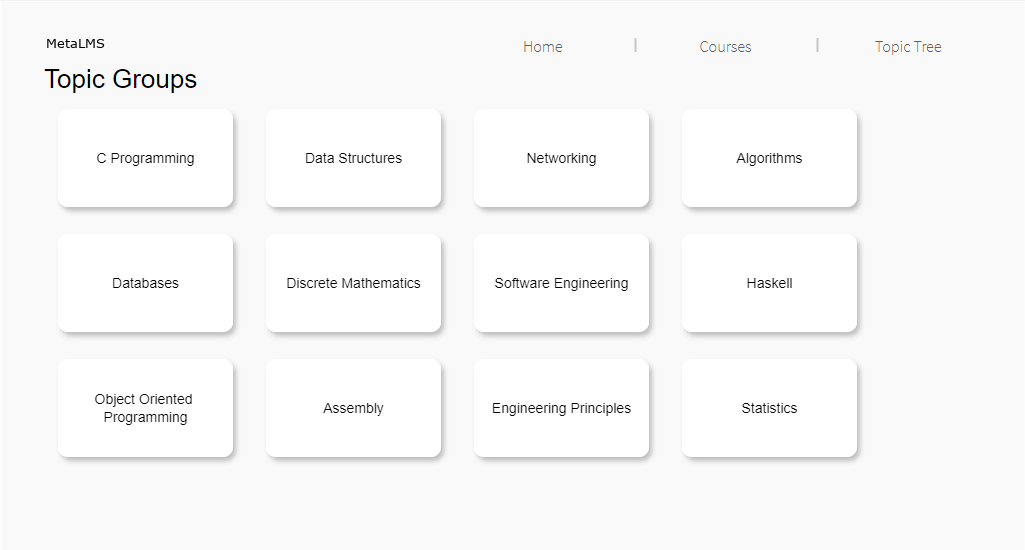
\includegraphics[scale=0.6]{topic-tree-groups-list}
    \caption{Topic Groups UI}
\end{figure}

Each group of topics is listed in card format. The topics in each group can be viewed by clicking on the topic.\\

\begin{figure}[h!]
    \centering
    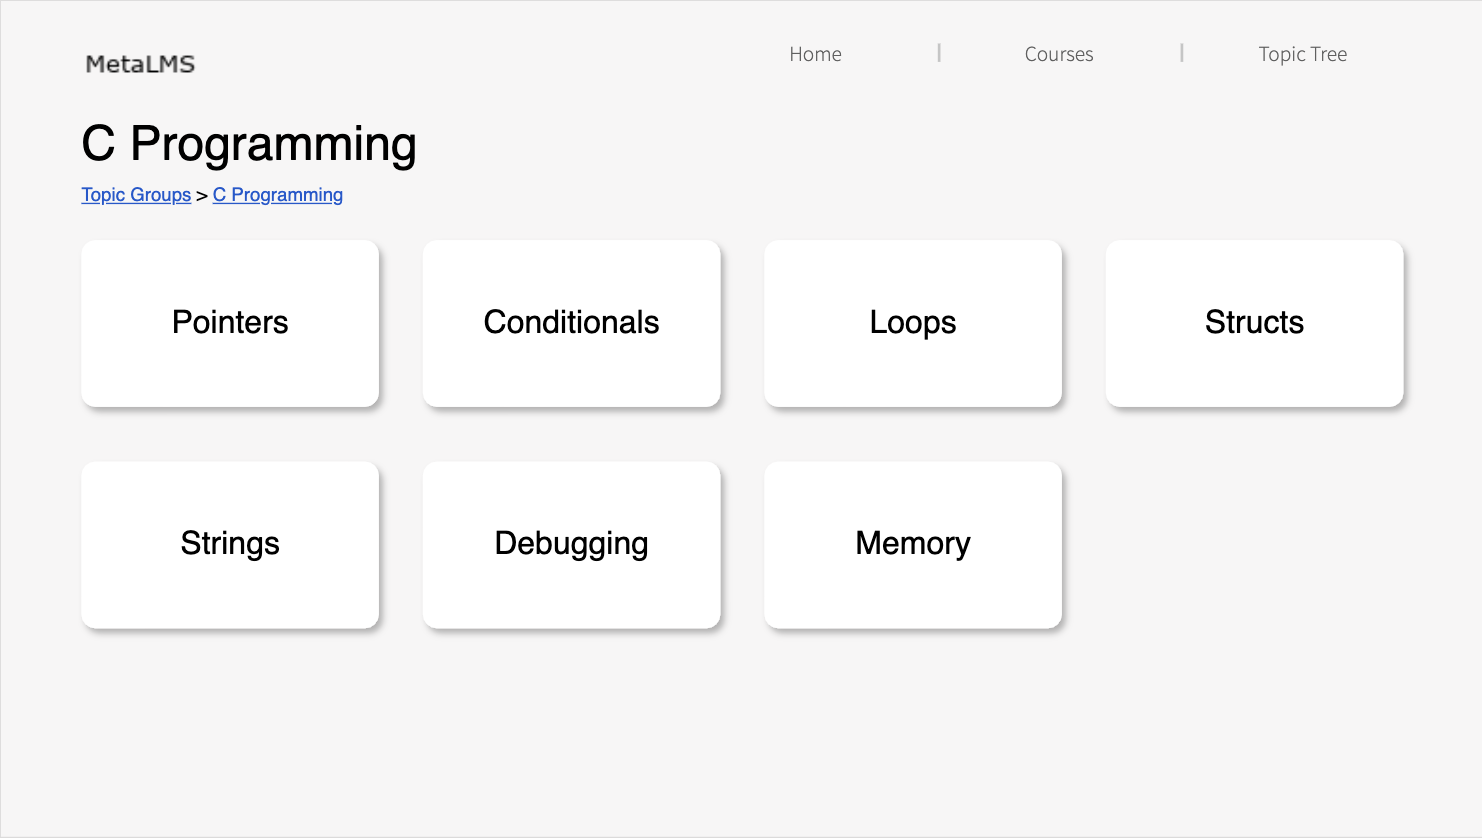
\includegraphics[scale=0.4]{topic-tree-group}
    \caption{Topic Group - C Programming Example}
\end{figure}
\newpage

Inside a topic group, the full list of topics inside this group is listed. Prerequisites are NOT shown here. \\

\begin{figure}[h!]
    \centering
    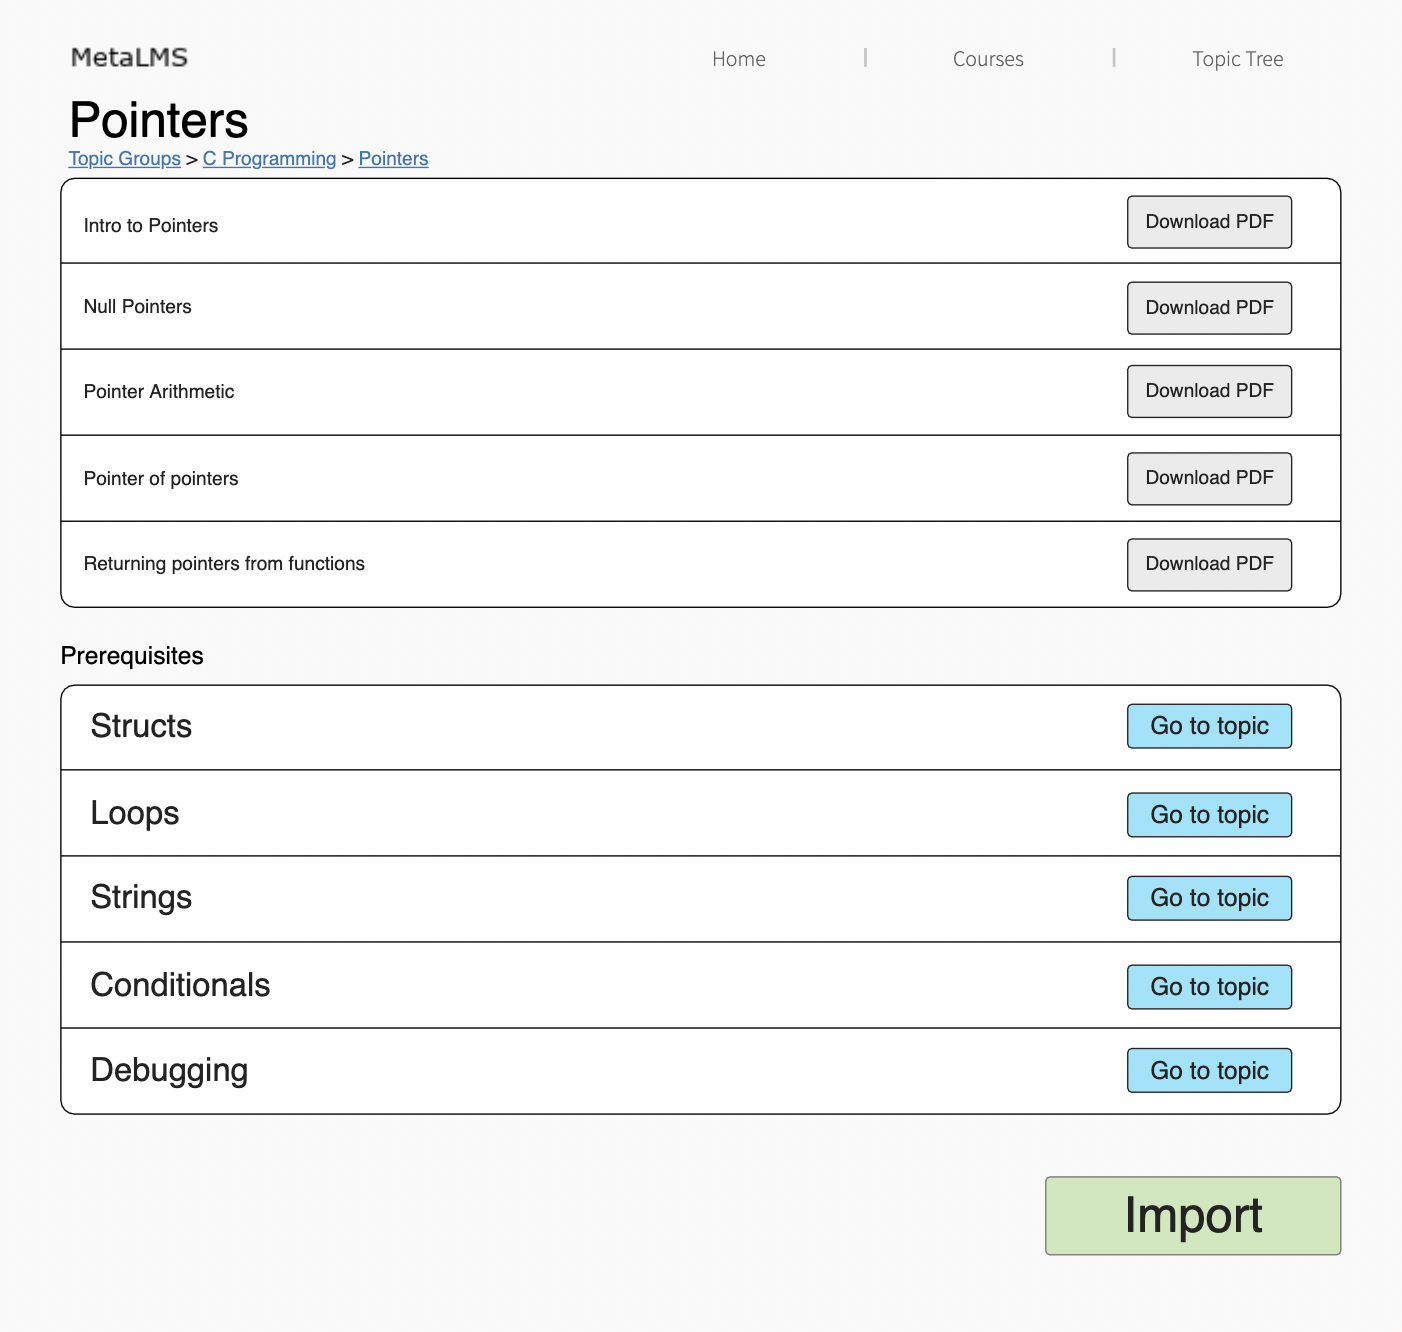
\includegraphics[scale=0.4]{topic-tree-pointers}
    \caption{Topic - Pointers Example}
\end{figure}

All resources for this topic are listed, and prerequisites are also listed on this page. This view is modelled after the UNSW handbook, where course prerequisites are listed as links. This topic can then be imported into a course with the import button at the bottom.\\

\subsection{Requirements}
The requirements below are draft requirements, and will become more specific throughout the next stages of the thesis.\\
Each requirement will have a priority: High, Medium or Low. High priority requirements will be completed first, and then medium and low priority requirements respectively. \\

\subsection{Functional Requirements}

\textbf{Viewing Topics}

    \begin{enumerate}
    \item Users can view groups of topics \textcolor{Orange}{Medium}
    \item Users can view topics within each group \textcolor{Red}{High}
    \item Users can search for a topic \textcolor{Red}{High}
    \item Users can search for specific resources \textcolor{Red}{High}
    \item Users can view topic prerequisites \textcolor{Orange}{Medium}
    \item Users can view a graph of topics and their prerequisites \textcolor{Blue}{Low}
    \end{enumerate}

\textbf{Adding Topics and resources}
    \begin{enumerate}
    \item Users can add a new topic \textcolor{Red}{High}
    \item Users can upload course material \textcolor{Red}{High}
    \item Users can add a new topic group \textcolor{Orange}{Medium}
    \end{enumerate}

\textbf{Deleting Topics}
    \begin{enumerate}
    \item Users can delete a topic that they've created \textcolor{Red}{High}
    \item Users can delete a topic group that they've created \textcolor{Orange}{Medium}
    \item Users can remove course material from a topic \textcolor{Red}{High}
    \end{enumerate}

\textbf{Topic Prequisites}
    \begin{enumerate}
    \item Users can add a topic prerequisite \textcolor{Orange}{Medium}
    \item Users can delete a topic prerequisite \textcolor{Orange}{Medium}
    \end{enumerate}

\textbf{Integration}
    \begin{enumerate}
    \item Users can import course material by selecting topics for a course \textcolor{Red}{High}
    \item Users can remove topics from a course \textcolor{Red}{High}
    \end{enumerate}

\textbf{Exporting}
    \begin{enumerate}
    \item Users can export data from topics and course material \textcolor{Blue}{Low}
    \end{enumerate}

\subsection{Timeline}
This timeline details what is planned over the course of the year to achieve a working topic tree feature in the meta learning management system.
Milestones are featured throughout this timeline.

\newpage

\begin{figure}[h!]
    \centering
    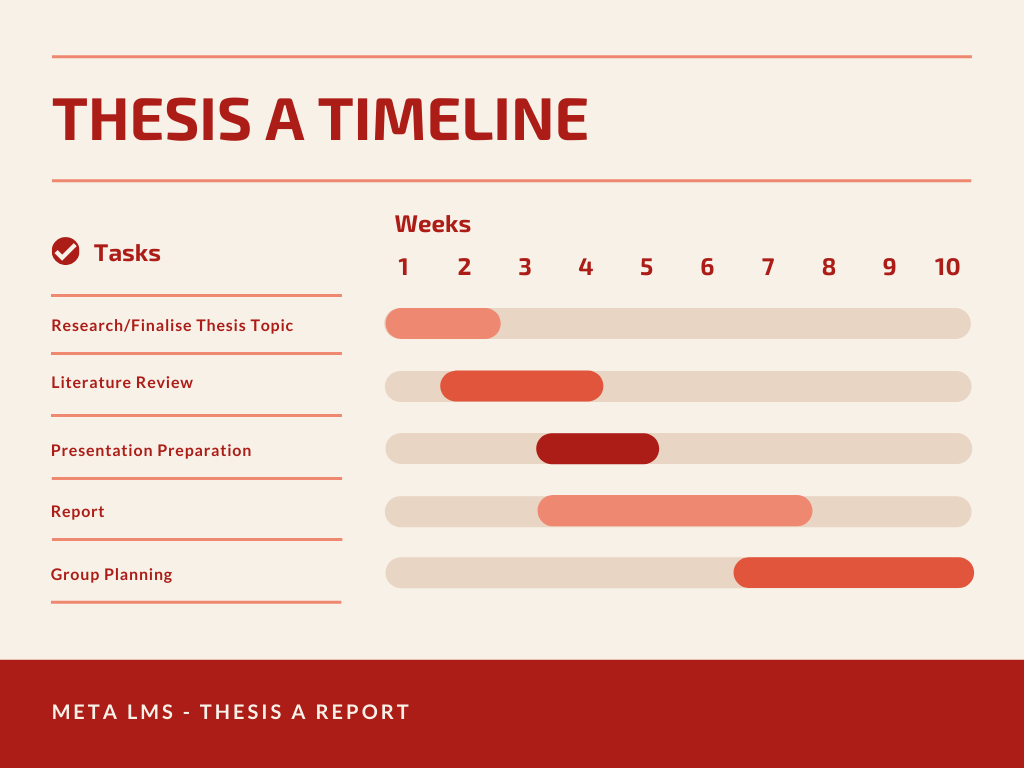
\includegraphics[scale=0.4]{topic-tree-thesis-a}
    \caption{Thesis A Timeline}
\end{figure}

This term, the focus is literature review and planning features for implementation in Thesis B and C.


\begin{figure}[h!]
    \centering
    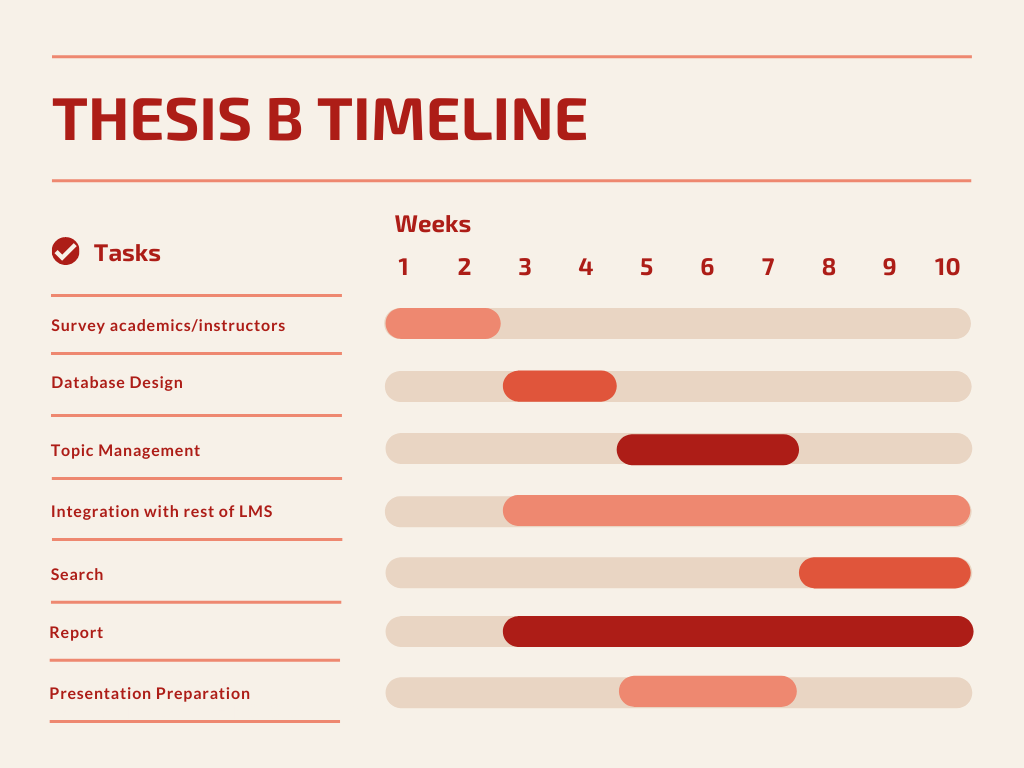
\includegraphics[scale=0.4]{topic-tree-thesis-b}
    \caption{Thesis B Timeline}
\end{figure}

In Thesis B, the focus is to start implementing the topic tree feature, with core features implemented and mostly usable, and a working database design. \\

Database Design will involve designing a schema for the database to store topics and their dependencies. This will most likely involve a graph relationship between topics.\\
Topic Management involves designing the interface for adding, removing and managing topics and helping develop a backend for this.\\
Integration with the rest of the system involves using the topic tree to import content into a course, and export content into the topic tree, etc.\\
Search involves searching for content, and is not as important as developing the topic management feature.\\

\begin{figure}[h!]
    \centering
    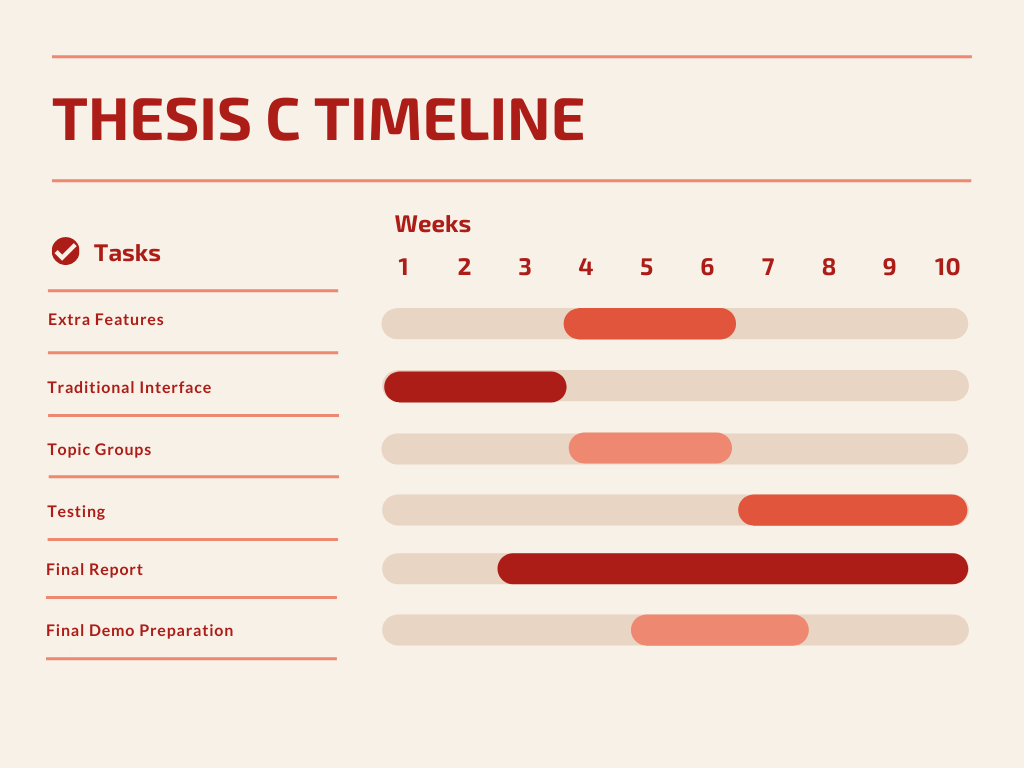
\includegraphics[scale=0.4]{topic-tree-thesis-c}
    \caption{Thesis C Timeline}
\end{figure}

In Thesis C, the main focus is to finalise features, fix any bugs that arise, test the feature and its integration with the rest of the system, implement a graph interface and allow topics to be grouped with each other.\\

A graph interface would make it much easier to visualise dependencies between topics, but is not a high priority so the plan is to implement this during Term 3 2021.\\

\newpage
\subsection{Milestones}
Major milestones for the topic tree feature include: \\
\begin{enumerate}
\item Week 6 Term 2 2021 - Implement a database schema for storing topics and their prerequisites, and set up an interface for topic management.
\item Week 11 Term 2 2021 - Adding and deleting topic prerequisites/dependencies, a search function and proper integration with the rest of the learning management system
\item Week 6 Term 3 2021 - Graph interface to easily view prerequisites between topics and topic groups
\item Week 11 Term 4 2021 - Final Testing and Analysis of the learning management system
\end{enumerate}

\subsection{Evaluation}
In order to evaluate how well the feature has met its requirements and achieved its purpose, a criteria will be proposed. In addition to meeting its requirements, the feature will also be assessed in several areas:
\begin{enumerate}
    \item Performance - Whether the topic tree feature is fast and responsive
    \item Accessibility - Can a wide array of users use the topic tree easily (including people with disabilities, etc.)
    \item UI/UX - Is the feature easy to use and attractive
    \item Errors - Is the feature bug and error free
\end{enumerate}